 \documentclass[11pt, oneside]{article}   	% use "amsart" instead of "article" for AMSLaTeX format
\usepackage{geometry}                		% See geometry.pdf to learn the layout options. There are lots.
\geometry{letterpaper}                   		% ... or a4paper or a5paper or ... 
%\geometry{landscape}                		% Activate for for rotated page geometry
%\usepackage[parfill]{parskip}    		% Activate to begin paragraphs with an empty line rather than an indent
\usepackage{graphicx}				% Use pdf, png, jpg, or eps§ with pdflatex; use eps in DVI mode
								% TeX will automatically convert eps --> pdf in pdflatex		
\usepackage{amssymb}
\usepackage{amsmath}
\usepackage{parskip}
\usepackage{color}
\usepackage{hyperref}

\title{Definitions}
%\author{The Author}
%\section{}
%\subsection*{}
\date{}							% Activate to display a given date or no date

\graphicspath{{/Users/telliott_admin/Dropbox/Tex/png/}}
% \begin{center} 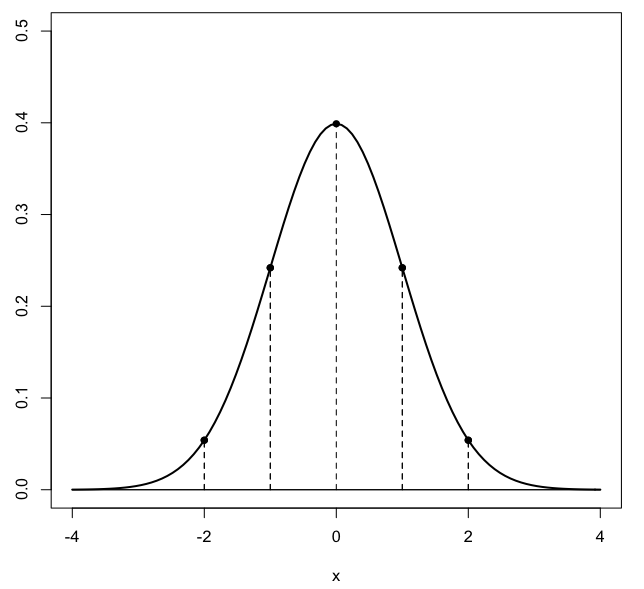
\includegraphics [scale=0.4] {gauss3.png} \end{center}
\begin{document}
\maketitle
\Large
\subsection*{Neighborhood}
A neighborhood or $\epsilon$ neighborhood of $z_0$ means simply all
\[ z:  |z - z_0| < \epsilon \]
\subsection*{Deleted neighborhood}
A deleted neighborhood does not include the point $z_0$:
\[ z:  0 < |z - z_0| < \epsilon \]

\subsection*{Limit}
Let a function $f$ be defined at all points $z$ in some deleted neighborhood of $z_0$, then the statement
\[ \lim_{z \rightarrow z_0} f(z) = w_0 \]
means that the point $w = f(z)$ can be made arbitrarily close to $w_0$ if we choose the point $z$ close enough to $z_0$ (though distinct from it).
  
Formally, for each positive number $\epsilon$, there exists a positive number $\delta$ such that
\[ |z - z_0| < \delta \ \ \Rightarrow |f(z) - w_0| < \epsilon \]
\begin{center} 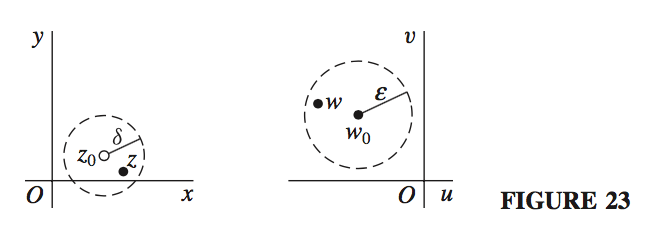
\includegraphics [scale=0.5] {Brown_Fig23.png} \end{center}
If the limit of a function exists at a point, it is unique.

\subsection*{Continuity}
A function $f$ is continuous as a point $z_0$ if all three conditions hold:
\[ \lim_{z \rightarrow z_0} f(z) = f(z_0) \]
which of course requires
\[ f(z_0) \text{ exists} \]
\[ \lim_{z \rightarrow z_0} f(z) \text{ exists} \]

\subsection*{Differentiable}
A function $f$ is said to be differentiable at if the function's domain includes a neighborhood of $z_0$ and the derivative exists:
\[ f'(z_0) = \lim_{z \rightarrow z_0} \frac{f(z) - f(z_0)}{z - z_0} \]
The existence of the derivative at $z_0$ implies that the function is continuous at that point;  however, the converse is not true.

\subsection*{Analytic}
A function is analytic at a point if it has a derivative at that point.

\subsection*{Entire}
An entire function is a function that is analytic at each point in the entire finite plane.

\subsection*{Singular point}
A point $z_0$ is called a singular point of a function $f$ if $f$ fails to be analytic at $z_0$  but is analytic at some point in every neighborhood of $z_0$ . 

A singular point $z_0$  is said to be isolated if, in addition, there is a deleted neighborhood  of $z_0$  throughout which $f$ is analytic.

\subsection*{Pole}
An isolated singular point is called a pole.  For example
\[ \frac{b_1}{z - z_0} \]
has a pole at $z_0$, since it is undefined there.  A pole of order $m$ would be
\[ \frac{b_1}{(z - z_0)^m} \]

\subsection*{Holomorphic and meromorphic}
Holomorphic is used as a synonym for analytic.  A function $f$ is said to be meromorphic in a domain $D$ if it is analytic throughout $D$ except for poles.

\subsection*{Limit of a sequence}
An infinite sequence of complex numbers $z_1 \dots z_n$ has a limit $L$ if, for each positive number $\epsilon$, there exists a positive integer $n_0$ such that $|z_n - L| < \epsilon$ whenever $n>n_0$.

\subsection*{Cauchy sequence}


\end{document}  
